\BiChapter{环流的大偏差原理}{Large deviations of cycle currents}
大偏差原理关系到随机过程中小概率事件的长时涨落行为 \cite{varadhan1984large,den2000large}。我们考察了经验环流的大偏差。既然假设周期边界条件,那么定义单环马氏链的经验LE环流$(J_n^c)_{c \in \mathcal{C}}$在空间:
\begin{equation*}
    \mathcal{V} = \left\{(\nu^c)_{c\in \mathcal{C}}:\;\nu^c\geq 0,\;
    \sum_{c\in \mathcal{C}}|c|\nu^c  = 1\right\},
\end{equation*}
其中$|c|$表示环$c$的长度,即环$c$中状态数量。若满足下列三个条件\cite{varadhan1984large},则称经验LE环流$(J_n^c)_{c \in \mathcal{C}}$满足速率函数为$I_J:\mathcal{V}\rightarrow [0,\infty]$的大偏差原理:
\begin{itemize}
    \item 对于$\forall \alpha \geqslant 0$,水平集$\{x \in \mathcal{V}: I_{J}(x) \leqslant \alpha\}$是紧的。
    \item 对于任意开集$U \subset \mathcal{V}$,
        \begin{equation}\label{def1}
            \varliminf_{n\to\infty}\frac{1}{n}\log\mathbb{P}((J^c_n)_{c\in\mathcal{C}}\in U)\ge-\inf_{x\in U}I_J(x).
        \end{equation}
    \item 对于任意闭集$F \subset \mathcal{V}$,
        \begin{equation}\label{def2}
            \varlimsup_{n\to \infty}\frac{1}{n}\log\mathbb{P}((J^c_n)_{c\in\mathcal{C}}\in F)\le -\inf_{x\in F}I_J(x).
        \end{equation}
\end{itemize}
从中可以看出,定义中的条件$(ii)$和$(iii)$表明,对任意 $(\nu^c)_{c\in\mathcal{C}}\in\mathcal{V}$,满足:
\begin{equation}\label{LDP}
    \mathbb{P}(J^c_n=\nu^c,\;\forall c\in\mathcal{C})\propto e^{-n I_J(\nu)},\;\;\;n\to\infty,
\end{equation}
同样地,也可以定义经验ST环流的大偏差$(Q_c^{c_l})_{l \subset \mathcal{L}}$。

\BiSection{单环马氏链LE环流的大偏差}{}
\BiSubsection{大偏差速率函数的基本推导}{}
首先我们讨论经验LE环流的大偏差原理。一般的马氏链中,速率函数的解析表达式$I_J$很难被求出,因此下面将研究单环马氏链。单环系统中所有可能形成的环都已在 (\ref{cycle_space})中列出。

下面假设系统都从状态$1$出发,这样会简化叙述步骤,且不会降低命题的适用性。为了求出速率函数$I_J$,需要计算LE经验环流的联合分布。对任意环$c=(i_1, i_2, \cdots, i_s)$,令$\gamma^c = p_{i_1i_2}p_{i_2i_3}\cdots p_{i_si_1}$表示沿该环所有转移概率的乘积。对任意满足$\sum_{c \subset \mathcal{C}} |c| k^c=n$的非负整数序列$k=(k^c)_{c\subset \mathcal{C}}$,由周期边界条件,我们可得经验LE环流的联合分布为:
\begin{equation}\label{joint}
    \begin{split}
    \mathbb{P}\left(J^c_n=\nu^c,\;\forall c\in\mathcal{C}\right)
    =&\;\mathbb{P}\left(N^c_n=k^c,\;\forall c\in\mathcal{C}\right)\\
    =&\;|G_n(k)|\prod_{c\in\mathcal{C}}\left(\gamma^c\right)^{k^c},
    \end{split}
\end{equation}
其中$\nu^c = k^c/n$,$G_n(k)$表示$n$时刻可能形成的轨道的集合,且称该类轨道为容许轨道。

为书写方便,若$c=(i)$是一元环,则用$k^i$替代$k^c$;若$c=(i,i+1)$是二元环,则用$k^{i,i+1}$表示;若$c=(1,2,\cdots,N)$是顺时针$N$状态环,则用$k^{+}$表示;若$c=(1,N,\cdots,2)$是逆时针$N$状态环,则用$k^{-}$表示。类似地,也用$\nu^i, \nu^{i,i+1}, \nu^+, \nu^-$表示相应的经验环流,$J^i, J^{i, i+1}, J^{+}, J^{-}$表示相应的经验净环流。例如,对于三状态马氏链,如果序列$k=(k^c)_{c\subset \mathcal{C}}$为:
\begin{equation} \label{trajectory_ex}
    k^3 = k^{12} = k^{23} = k^- = 1, ~~~ k^1 = k^2 = k^{13} = k^+= 0
\end{equation}
那么在时刻$n=8$,有8个容许轨道,如表\ref{table:all possible trajectories}所示。

\begin{table}[htb!]
    \renewcommand\arraystretch{0.8}
    \begin{tabular}{cccccccccc}
    \hline
   $m$   & 0 & 1 & 2 & 3 & 4 & 5 & 6 & 7 & 8 \\\hline
   $\xi_m$& 1 & 3 & 3 & 2 & 3 & 2 & 1 & 2 & 1 \\\hline
   $\xi_m$& 1 & 3 & 2 & 3 & 3 & 2 & 1 & 2 & 1 \\\hline
   $\xi_m$& 1 & 3 & 3 & 2 & 1 & 2 & 3 & 2 & 1 \\\hline
   $\xi_m$& 1 & 3 & 2 & 1 & 2 & 3 & 3 & 2 & 1 \\\hline
   $\xi_m$& 1 & 2 & 3 & 3 & 2 & 1 & 3 & 2 & 1 \\\hline
   $\xi_m$& 1 & 2 & 3 & 2 & 1 & 3 & 3 & 2 & 1 \\\hline
   $\xi_m$& 1 & 2 & 1 & 3 & 3 & 2 & 3 & 2 & 1 \\\hline
   $\xi_m$& 1 & 2 & 1 & 3 & 2 & 3 & 3 & 2 & 1 \\\hline
    \end{tabular}\centering
    \caption{三状态马氏链中,8个容许轨道,环$(3), (12), (23)$和$(1,3,2)$形成一次,环$(1), (2), (13)$和$(1,2,3)$没有形成过}
    \label{table:all possible trajectories}
\end{table}

接下来计算容许轨道的数量$G_n(k)$。基本的思路是在近似有序的轨道中插入各种环,插入方式的数量将会是容许轨道的数量。计算过程分为三个步骤:

1)由于系统从状态$1$出发,作为第一步,选出所有包含初始状态$1$的环,即$(1)$,$(1,2)$,$(1,N)$,$(1,2,\cdots,N)$,$(1,N,\cdots,2)$,并且插入到轨道中。因为环$c$形成$k^c$次,所以步骤1)中插入方式的数量,也就是环的排列数为:
\begin{equation*}\label{formula:A1}
    A_1 = \binom{k^1+k^{12}+k^{1N}+k^{+}+k^{-}}{k^1,k^{12},k^{1N},k^{+},k^{-}}
    := \frac{(k^1+k^{12}+k^{1N}+k^{+}+k^{-})!}{k^1!\;k^{12}!\;k^{1N}!\;k^{+}!\;k^{-}!}.
\end{equation*}
对于 \ref{trajectory_ex}中的例子,步骤1)中所有可能的插入方式为图 \ref{figure:insertion}左部分所示。
\begin{figure}[htb!]
\centering
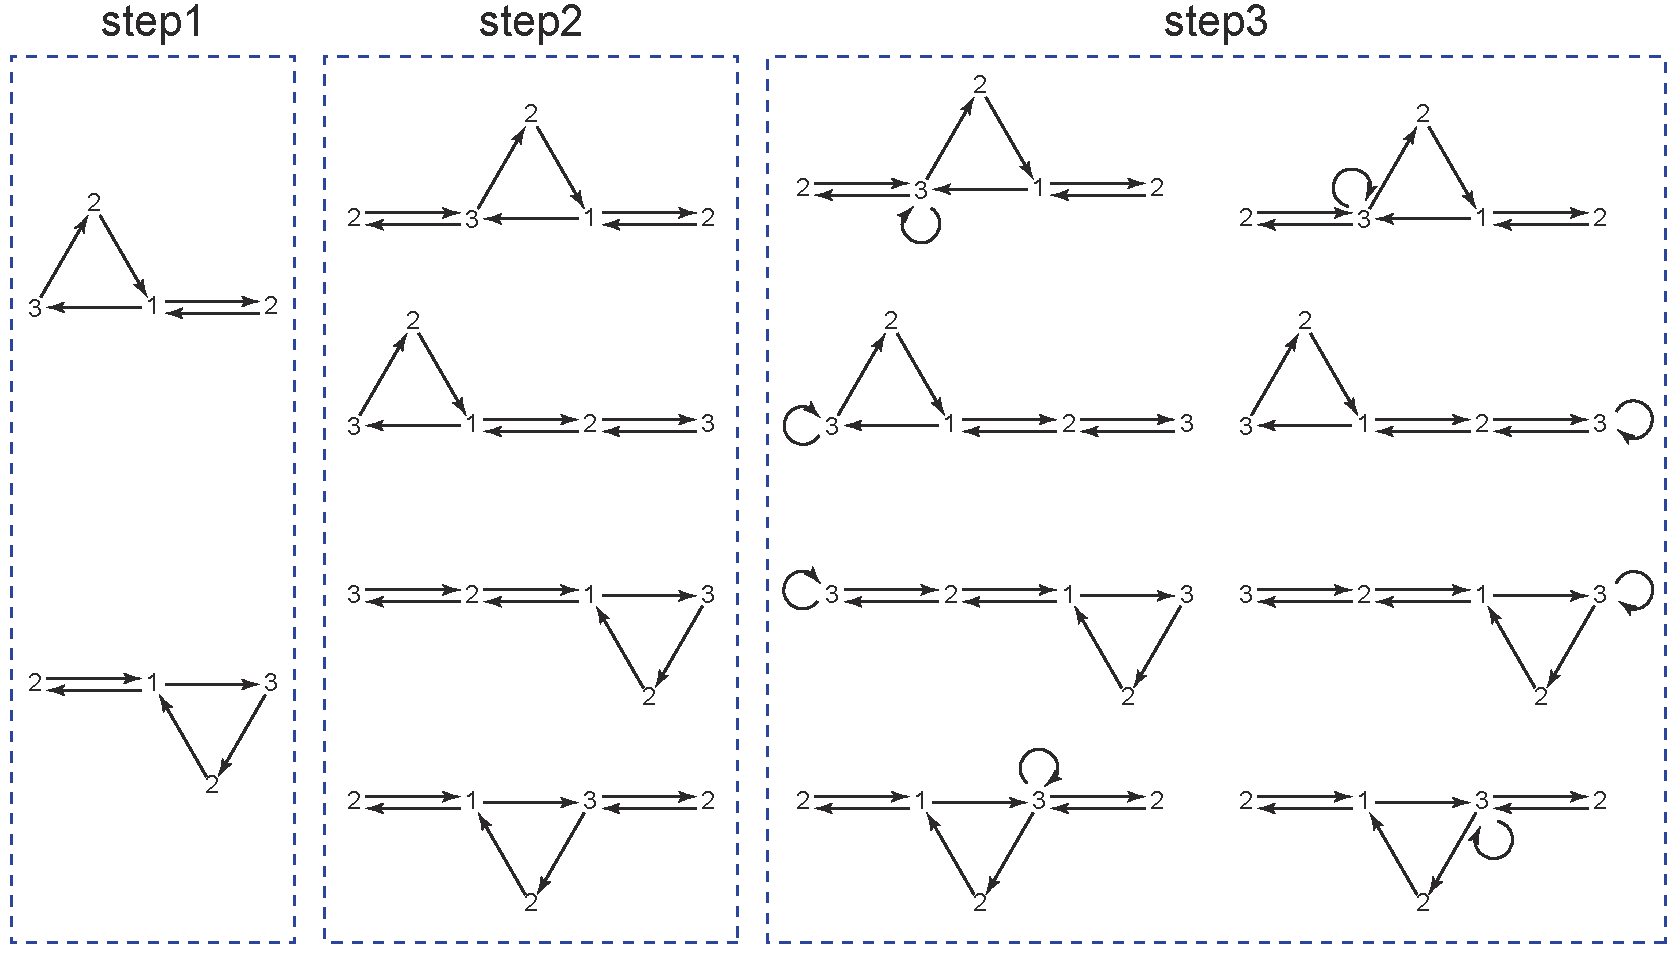
\includegraphics[scale=0.6]{chart/insertiongraph.pdf}
\caption{构建所有容允许轨道的环插入法示意图。依然使用\ref{trajectory_ex}中的例子。环插入法分为三步:首先我们将所有包含初始状态的环插入轨道,接下来我们将所有剩余的两元环插入轨道,最后我们将所有剩余的一元环插入轨道。经过这三步的环插入,找到了所有八个容许轨道,这与表中列出的轨道完全吻合。}
\label{figure:insertion}
\end{figure}

2)在轨道中插入剩余的二元环。仔细观察系统形成环$(i,i+1)$的情况,可能是在状态$i$,也可能是$i+1$。例如,轨道$\{1, 3, 2, 3, \cdots\}$,形成环$(2,3)$时,导出链是$[1, 3]$。因此,我们称该环是在状态$3$处形成。作为对比,轨道$\{1,2,3,2, \cdots\}$,形成环$(2,3)$时,导出链是$[1, 2]$,因此称该环是在状态$2$处形成的。

考虑两状态环$(i, i+1), 2\leqslant i \leqslant N-1$,记$l^i$和$m^i$分别表示在状态$i$和$i+1$处形成环$(i, i+1)$的数量,显然$l^i + m^i = k^{i, i+1}$。固定$l^i$和$m^i$的值,可以计算出相应的容许轨道数量。首先,在状态$2$处插入$l^2$个环$(2, 3)$,总共有$k^+ + k^{12}$个位置可以插入,然而环$(1,2, \cdots, N)$和环$(1, 2)$已经在步骤1)中考虑。既然这些位置没有包含环$(1, N, \cdots, 2)$中的状态$2$,如果插入$(2,3)$,那么这个环将会在状态$3$处形成,而不是状态$2$。因此插入方式的数量是:
\begin{equation} \label{binom1}
    \binom{k^++k^{12}+l^{2}-1}{l^{2}}.
\end{equation}
接下来,考虑状态$3 \leqslant i \leqslant N$对应的$l^i$个环,即$(i, i+1)$。把它们插入轨道中,其中每个状态$i$有$k^+ + l^{i-1}$个可能的位置插入,也就是环$(1, 2, \cdots, N)$和环$(i-1, i)$中的位置。因此总共插入方式数量是:
\begin{equation} \label{binom2}
    \binom{k^++l^{i-1}+l^{i}-1}{l^{i}},\;\;\;3\le i\le N-1.
\end{equation}
目前,已经插入$l^i$个环$(i,i+1)$。结合 \ref{binom1}和 \ref{binom2},所有的插入方式的数量是:
\begin{equation*}
    \prod_{i=2}^{N-1}\binom{l^{i}+l^{i-1}+k^{+}-1}{l^{i}}
\end{equation*}
其中$l^1:=k^{12}$。

同理,把状态$2 \leqslant i \leqslant N-1$对应的$m^i$个环$(i, i+1)$插入轨道,所有的插入方式的数量:
\begin{equation*}
    \prod_{i=2}^{N-1}\binom{m^{i}+m^{i+1}+k^{-}-1}{m^{i}},
\end{equation*}
其中$m^N:=k^{N1}$。所有两状态的环就已经完全被插入。步骤 2)中所有插入方式数量为:
\begin{equation*}
    A_2 = \sum_{l^{2}+m^{2}=k^{23}}\dots\sum_{l^{N-1}+m^{N-1}=k^{N-1,N}}
    \prod_{i=2}^{N-1}\binom{l^{i}+l^{i-1}+k^{+}-1}{l^{i}}\prod_{i=2}^{N-1}\binom{m^{i}+m^{i+1}+k^{-}-1}{m^{i}},
\end{equation*}
例子 \ref{trajectory_ex}中,步骤2)中的插入方式在图 \ref{figure:insertion}的中间部分。

3)最后把所有剩余的一元环插入轨道中。对每个环$(i), 2 \leqslant i \leqslant N$,有$\sum_{c\ni i}k^c-k^i$个可选择的位置插入。步骤 3)总共的插入方式数量为:
\begin{equation*}\label{formula:A3}
    A_3 = \prod_{i=2}^N\binom{\sum_{c\ni i}k^{c}-1}{k^{i}}.
\end{equation*}
例子 \ref{trajectory_ex}中,步骤3)的插入方式在图 \ref{figure:insertion}的右部分。

结合上述三个步骤,可以得到容许轨道的数量为:$|G_n(k)|=A_1A_2A_3$。因此LE经验环流的联合分布为:
\begin{equation} \label{trajectories}
    \mathbb{P}\left(J^c_n=\nu^c,\;\forall c\in\mathcal{C}\right)
    = A_1 A_2 A_3 \Pi_{c\in\mathcal{C}} (\gamma^c)^{K^c}
\end{equation}
为了得到更明确的速率函数表达式$I_J$,我们回顾$Stirling$公式:
\begin{equation*}
    \log n! = n\log n-n+O(\log n)=h(n)-n+O(\log n),
\end{equation*}
其中$h(x)=x \log x, x \geqslant 0$。记$k_i=\sum_{c\ni i}k^c$且$\nu_i=\sum_{c\ni i}\nu^c$,注意到$k_i$和$k^i$的定义是不同的,由$Stirling$可得:
\begin{equation}\label{log A1}
    \begin{split}
    \log A_1&=\log\frac{(k^1+k^{12}+k^{1N}+k^{+}+k^{-})!}{k^1!\;k^{12}!\;k^{1N}!\;k^{+}!\;k^{-}!}\\
    &= h(k_1)-h(k^1)-h(k^{12})-h(k^{1N})-h(k^+)-h(k^-)+O(\log n)\\
    &= n\left[h(\nu_1)-h(\nu^1)-h(\nu^{12})-h(\nu^{1N})-h(\nu^+)-h(\nu^-)\right]+O(\log n).
    \end{split}
\end{equation}
类似地,有:
\begin{equation}\label{log A3}
    \begin{split}
    \log A_3&=\log\left[\prod_{i=2}^N\binom{k_i-1}{k^{i}}\right]
    =\sum_{i=2}^N\log\left(\frac{\left(k_i\right)!}{\left(k^i\right)!\left(k_i-k^i\right)!}\right)+O(\log n)\\
    &=\sum_{i=2}^N\left[h(k_i)-h(k^i)-h(k_i-k^i)\right]+O(\log n)\\
    &=\sum_{i=2}^Nn\left[h(\nu_i )-h(\nu^i)-h(\nu_i-\nu^i)\right]+O(\log n).
    \end{split}
\end{equation}
最后,估计$\log A_2$,令$D = \{(l^i,m^i)_{2\le i\le N-1}:\;l^i,m^i\in\mathbb{N},\;l^i+m^i=k^{i,i+1}\}$ 表示$l^i$和$m^i$的组合形成的集合。记$L = (l^i,m^i)\in D$, 令
\begin{equation*}
    B_L=\prod_{i=2}^{N-1}\binom{l^{i}+l^{i-1}+k^{+}-1}{l^{i}}\binom{m^{i}+m^{i+1}+k^{-}-1}{m^{i}}.
\end{equation*}
表示在给定$l^i$和$m^i$时,步骤 2)中插入方式的数量。易知$|D| \leqslant n^{N-2}$,因此,可得:
\begin{equation}\label{inequality}
    \max_{L\in D}B_L \le A_2 \le (n+1)^{N-2} \max_{L\in D}B_L,
\end{equation}
该式中还使用了结论$A_2 = \sum_{L\in D}B_L$。类似于 \ref{log A3} 式,有:
\begin{equation}\label{log BL}
    \begin{split}
    \log B_L =&\;\sum_{i=2}^{N-1}[h(l^i+l^{i-1}+k^+)-h(l^i)-h(l^{i-1}+k^+)]\\
    &\;+\sum_{i=2}^{N-1}[h(m^i+m^{i+1}+k^-)-h(m^i)-h(m^{i+1}+k^-)]+O(\log n)\\
    =&\;\sum_{i=2}^{N-1}n[h(x^i+x^{i-1}+\nu^+)-h(x^i)-h(x^{i-1}+\nu^+)]\\
    &\;+\sum_{i=2}^{N-1}n[h(y^i+y^{i+1}+\nu^-)-h(y^i)-h(y^{i+1}+\nu^-)]+O(\log n),
    \end{split}
\end{equation}
其中$x^i = l^i/n$和$y^i = m^i/n$。对于任意的$\nu \in \mathcal{V}$,考虑空间:
\begin{equation*}
    V(\nu) = \left\{\left(x^{i},y^{i}\right)_{2\le i\le N-1}:\;x^i,y^i\geq0,\;x^{i}+y^{i}=\nu^{i,i+1}\right\},
\end{equation*}
且对任意$X = (x^i, y^i) \in V(\nu)$。定义函数:
\begin{equation}\label{formula:F}
    \begin{split}
    F_{\nu}(X)
    =&\sum_{i=2}^{N-1}\left[ h\left(x^{i-1}+\nu^+\right) + h\left(x^{i}\right) - h\left(x^{i-1}+x^{i}+\nu^+\right) \right] \\
    &+ \sum_{i=2}^{N-1} \left[h\left(y^{i}\right) + h\left(y^{i+1} +\nu^-\right)-h\left(y^{i} +y^{i+1} +\nu^-\right)\right].
    \end{split}
\end{equation}
其中$x^1=\nu^{12}$,$y^N=\nu^{N1}$,再由式联系 \ref{inequality}的结论,可得:
\begin{equation}\label{log A2}
    \log A_2 = \max_{L\in D}\log B_L+O(\log n)
    = n\sup_{X\in V(\nu)}F_{\nu}(X)+O(\log n).
\end{equation}
结合\eqref{LDP}和\eqref{trajectories},可得:
\begin{equation*}
    \begin{split}
    I_J(\nu) &= -\lim_{n\to\infty}\frac{1}{n}\log\mathbb{P}\left(J^c_n=\nu^c,\;\forall c\in\mathcal{C}\right)\\
    &= -\lim_{n\to\infty}\frac{1}{n}\left[\log A_1+\log A_2+\log A_3+\sum_{c\in\mathcal{C}}k^c\log\gamma^c\right].
    \end{split}
\end{equation*}
再联系\eqref{log A1}, \eqref{log A3} 和 \eqref{log A2}式,可得:
\begin{equation}\label{ratefunction}
    \begin{split}
    I_J(\nu) =&\; \left[h\left(\nu^{12}\right)+h\left(\nu^{1N}\right)
    +h\left(\nu^+\right)+h\left(\nu^-\right)-h\left(\nu^{12}+\nu^{1N}+\nu^++\nu^-\right)\right] \\
    &\;+\inf_{X\in V(\nu)}F_{\nu}(X)+\sum_{i\in S}\left[ h\left(\nu_i-\nu^i\right)+h\left(\nu^i\right)
    -h\left(\nu_i\right)\right]-\sum_{c\in\mathcal{C}}\nu^c\log\gamma^c,
    \end{split}
\end{equation}
其中$h(x) = x \log x$,$\nu_i=\sum_{c\ni i}\nu^c$。这就是LE经验完整的环流速率函数表达式。该式中的$\inf_{X\in V(\nu)}F_{\nu}(X)$难以直接计算,下面将会介绍如何通过拉格朗日乘子法把该优化问题转化为代数方程求解的问题,即证明:
\begin{equation*}
    \inf_{X\in V(\nu)}F_{\nu}(X) = F_{\nu}(x^i,y^i),
\end{equation*}
其中$(x^i,y^i)_{2\leq i\leq N-1}$是下面代数方程的解:
\begin{equation}\label{equation}
    \begin{split}
    \frac{x^{i}}{x^{i-1}+x^{i}+\nu^+}\cdot\frac{x^{i}+\nu^+}{x^{i}+x^{i+1}+\nu^+}
    &= \frac{y^{i}+\nu^-}{y^{i-1}+y^{i}+\nu^-}\cdot\frac{y^{i}}{y^{i}+y^{i+1}+\nu^-},\\
    x^{i} + y^{i} &= \nu^{i,i+1},
    \end{split}
\end{equation}
这里$x^1=\nu^{12}$,$x^N=0$,$y^1=0$,且$y^N=\nu^{1N}$。

%%%%%%%%%%%%%%%%%%%%%%%%%%%%%%%%%%%%%%%%%%%%%%%%%%%%%%%%%%%%%%%%%%%%%%%%%%%%%%
% \subsubsection{附录 A:单环马氏链速率函数 $I_J$ 的表达式 }{} \label{appendix:explicit}
% 回顾单环系统,LE经验净环流$(J_n^c)_{c \in \mathcal{C}}$的速率函数为:
% \begin{equation*}\label{ratefunction2}
% 	\begin{split}
% 		I_J(\nu) =&\; \left[h\left(\nu^{12}\right)+h\left(\nu^{1N}\right)
% 		+h\left(\nu^+\right)+h\left(\nu^-\right)-h\left(\nu^{12}+\nu^{1N}+\nu^++\nu^-\right)\right] \\
% 		&\;+\inf_{X\in V(\nu)}F_{\nu}(X)+\sum_{i\in S}\left[ h\left(\nu_i-\nu^i\right)+h\left(\nu^i\right)
% 		-h\left(\nu_i\right)\right]-\sum_{c\in\mathcal{C}}\nu^c\log\gamma^c,
% 	\end{split}
% \end{equation*}
% % 下面将使用拉格朗日乘子法化简该式。固定 $\nu\in\mathcal{V}$,令拉格朗日函数 \cite{brian1990optimization} $\mathcal{A}_{\nu}:V(\nu)\times \mathbb{R}^{N-2}\to \mathbb{R}$ 为:
% 这里$\inf_{X\in V(\nu)}F_{\nu}(X)$不是闭形式,下面利用拉格朗日乘子法求解$\inf_{X\in V(\nu)}F_{\nu}(X)$。

首先我们定义拉格朗日函数为:
\begin{align*}
    \mathcal{A}_{\nu}(X,\lambda) = F_{\nu}(X) + \sum_{i=2}^{N-1} \lambda_i \left(x^{i} + y^{i} - \nu^{i,i+1}\right), \;\;\;\forall \nu\in\mathcal{V}
\end{align*}
其中 $X=(x^i,y^i)_{2\le i\le N-1}\in V(\nu)$ 并且 $\lambda=(\lambda_i)_{2\le i\le N-1}\in \mathbb{R}^{N-2}$。然后,分别对 $x^{i}$,$y^{i}$ 和 $\lambda_i$求导,可以得到下列方程:
\begin{equation}\label{equation1}
	\begin{split}
		\log\left(x^{i}\right) - \log\left(x^{i-1}+x^{i}+\nu^{+}\right)  + \log\left(x^{i}+\nu^{+}\right) -\log\left(x^{i}+x^{i+1}+\nu^{+}\right)+\lambda_i  &= 0, \\
		\log\left(y^{i}+\nu^{-}\right) -\log\left(y^{i-1}+y^{i}+\nu^{-}\right)  + \log\left(y^{i}\right) - \log\left(y^{i}+y^{i+1}+\nu^{-}\right) +\lambda_i &= 0, \\
		x^{i} + y^{i} = \nu^{i,i+1},\qquad 2\le i\le N-1.\qquad\qquad\qquad
	\end{split}
\end{equation}
我们可以把方程组 \eqref{equation1} 写为:
\begin{equation}\label{equations}
    \begin{split}
    \frac{x^{i}}{x^{i-1}+x^{i}+\nu^+}
    \,\frac{x^{i}+\nu^+}{x^{i}+x^{i+1}+\nu^+}
    &= \frac{y^{i}+\nu^-}{y^{i-1}+y^{i}+\nu^-}
    \,\frac{y^{i}}{y^{i}+y^{i+1}+\nu^-}=e^{-\lambda_i},\\
    x^{i} + y^{i} &= \nu^{i,i+1},\qquad 2\le i\le N-1.
    \end{split}
\end{equation}
其中 $x^1=\nu^{12}$,$x^N=0$,$y^1=0$ 和 $y^N=\nu^{1N}$。
\\

\begin{lemma}\label{lemma:existence for equations solution}
	方程 \eqref{equations} 有解 $X=(x^i,y^i)\in V(\nu)$。
\end{lemma}
\begin{proof}
    若对某些 $2\le k\le N-1$ 存在 $\nu^{k,k+1}=0$,则有 $x^{k}=y^{k}=0$ 成立。那么依据 $2\le i\le k-1$ 和 $k+1\le i\le N-1$,方程 \eqref{equations} 可以被分为两个方程。因此对于 $\nu^{k,k+1}>0, \forall k, 2\le k\le N-1$,下面会从三种不同情况考虑该引理。

    情况 1:$\nu^{12}=\nu^{+}=\nu^{1N}=\nu^-=0$。
    易知,对任意 $\alpha\in (0,1)$,
    \begin{equation*}
        x^{i}=\alpha\nu^{i,i+1},\quad y^{i}=(1-\alpha)\nu^{i,i+1},\quad 2\le i\le N-1,
    \end{equation*}
    都是 \eqref{equations} 的解。

    情况 2:$\nu^{12}=\nu^{+}=0,\nu^{1N}+\nu^{-}>0$ 或 $\nu^{1N}=\nu^{-}=0,\nu^{12}+\nu^{+}>0$。容易验证若 $\nu^{12}=\nu^{+}=0,\nu^{1N}+\nu^{-}>0$成立,则$x^{i}=0,y^{i}=\nu^{i,i+1}$ 是方程 \eqref{equations} 的解。

    情况 3:$\nu^{12}+\nu^{+}>0$ 或 $\nu^{1N}+\nu^{-}>0$。我们已经证明了对任意$2\le i\le k$,只要$x^{k+1}\ge 0$,$y^{k+1}>0$,和 $x^{k+1}+y^{k+1}=\nu^{k+1,k+2}$,存在满足下列方程的解:
    \begin{equation}\label{equations2}
        \begin{split}
            \frac{x^{i}}{y^{i}}
            =&\frac{x^{i}+x^{i+1}+\nu^+}{x^{i}+\nu^+}\, \frac{y^{i}+\nu^-}{y^{i-1}+y^{i}+\nu^-}
            \,\frac{x^{i-1}+x^{i}+\nu^+}{y^{i}+y^{i+1}+\nu^-},\\
            &\qquad x^{i} + y^{i} = \nu^{i,i+1},\qquad 2\le i\le k.
        \end{split}
    \end{equation}
    并且这个方程的解也满足$x^i,y^i,\; 2 \le i\le k$。下面通过归纳法证明,若 $k=2$,方程 \eqref{equations2} 可以简化为:
    \begin{equation*}\label{equation k=2}
        \frac{x^{2}}{\nu^{23}-x^2}
        =\frac{x^{2}+x^{3}+\nu^+}{x^{2}+\nu^+}\, \frac{\nu^{12}+x^{2}+\nu^{+}}{\nu^{23}-x^2+y^3+\nu^-}.
        %,\qquad \nu^+_{23} + \nu^-_{23} = \nu_{23}.
    \end{equation*}
    易得:
    \begin{equation*}
        \lim_{x^{2}\downarrow 0}\frac{x^{2}}{\nu^{23}-x^2} = 0,\qquad \lim_{x^{2}\downarrow 0}\frac{x^{2}+x^{3}+\nu^+}{x^{2}+\nu^+}\,  \frac{\nu^{12}+x^{2}+\nu^{+}}{\nu^{23}-x^2+y^3+\nu^-} \ge  \frac{\nu^{12}+\nu^{+}}{\nu^{23}+y^{3}+\nu^-} > 0.
    \end{equation*} 
    另外,有
    \begin{equation*}
        \lim_{x^2\uparrow \nu^{23}}\frac{x^{2}}{\nu^{23}-x^2} = \infty,\qquad \lim_{x^{2}\uparrow \nu^{23}}\frac{x^{2}+x^{3}+\nu^+}{x^{2}+\nu^+}\, \frac{\nu^{12}+x^{2}+\nu^{+}}{\nu^{23}-x^2+y^3+\nu^-} =  \frac{\nu^{23}+x^{3}+\nu^+}{\nu^{23}+\nu^+}\frac{\nu^{12}+\nu^{23}+\nu^{+}}{y^{3}+\nu^-} < \infty.
    \end{equation*}
    通过中值定理,可以找到满足 $x^{2},y^2>0$ 的方程 \eqref{equations2} 的解,并且有 $x^{2}+y^{2}=\nu^{2,3}$ 。假设对 $k=n-1$ 命题成立,那么可以考虑方程:
    \begin{equation*}
        \frac{x^{n}}{\nu^{n,n+1}-x^{n}} = \frac{x^{n}+x^{n+1}+\nu^+}{x^{n}+\nu^+}\,\frac{\nu^{n,n+1}-x^{n}+\nu^-}{y^{n-1}+\nu^{n,n+1}-x^{n}+\nu^-}\,\frac{x^{n-1}+x^{n}+\nu^+}{\nu^{n,n+1}-x^{n}+y^{n+1}+\nu^-},
    \end{equation*}
    其中 $x^{n-1}$, $y^{n-1}$ 是方程 \eqref{equations2} 在 $k=n-1$ 时的解。可以得到:
    \begin{equation}\label{limit1}
        \lim_{x^{n}\downarrow 0}\frac{x^{n}}{\nu^{n,n+1}-x^{n}}=0,
    \end{equation}
    并且
    \begin{equation}\label{limit2}
        \begin{split}
            &\;\lim_{x^{n}\downarrow 0}\frac{x^{n}+x^{n+1}+\nu^+}{x^{n}+\nu^+}\,\frac{\nu^{n,n+1}-x^{n}+\nu^-}{y^{n-1}+\nu^{n,n+1}-x^{n}+\nu^-}\,\frac{x^{n-1}+x^{n}+\nu^+}{\nu^{n,n+1}-x^{n}+y^{n+1}+\nu^-}\\
            \ge &\;\frac{\nu^{n,n+1}+\nu^-}{\lim_{x^{n}\downarrow 0}(y^{n-1})+\nu^{n,n+1}+\nu^-}\,\frac{\lim_{x^{n}\downarrow 0}(x^{n-1})+\nu^+}{\nu^{n,n+1}+y^{n+1}+\nu^-}>0.
        \end{split}
    \end{equation}
    利用归纳法得出的结论 $\lim_{x^{n}\downarrow 0}(x^{n-1})>0$,可以得到下面两个式子成立。
    \begin{equation}\label{limit3}
        \lim_{x^{n}\uparrow \nu^{n,n+1}}\frac{x^{n}}{\nu^{n,n+1}-x^{n}}=\infty,
    \end{equation}
    和
    \begin{equation}\label{limit4}
        \begin{split}
            &\;\lim_{x^{n}\uparrow \nu^{n,n+1}}\frac{x^{n}+x^{n+1}+\nu^+}{x^{n}+\nu^+}\,\frac{\nu^{n,n+1}-x^{n}+\nu^-}{y^{n-1}+\nu^{n,n+1}-x^{n}+\nu^-}\,\frac{x^{n-1}+x^{n}+\nu^+}{\nu^{n,n+1}-x^{n}+y^{n+1}+\nu^-}\\
            \le &\;\frac{\nu^{n,n+1}+x^{n+1}+\nu^+}{\nu^{n,n+1}+\nu^+}\,\frac{\lim_{x^{n}\uparrow \nu^{n,n+1}}x^{n-1}+\nu^{n,n+1}+\nu^+}{y^{n+1}+\nu^-}<\infty.
        \end{split}
    \end{equation}
    通过中值定理,可以找到方程 \eqref{equations2} 满足条件 $x^{i},y^i>0, x^{i}+y^{i}=\nu^{i,i+1}, \forall i=2,3, \cdots, n$ 的解。由归纳法,可以得到命题对 $k\ge 2$ 成立。

    既然 $k=N-1$时,方程 \eqref{equations2} 与 方程 \eqref{equations} 等价。这时。有$y^{k+1}=y^N=\nu^{1N}$。由于$\nu^{N1}+\nu^->0$,易知\eqref{limit1},\eqref{limit2},\eqref{limit3} 和 \eqref{limit4} 成立。类似上述证明,通过中值定理,找到方程 \eqref{equations2} 满足条件 $x^{i},y^i>0, x^{i}+y^{i}=\nu^{i,i+1}, \forall i=2,3, \cdots, n$ 的解。证毕。
\end{proof}

\begin{lemma}\label{lemma:mininum}
    令 $X=(x^i,y^i)\in V(\nu)$ 是引理 ~\ref{lemma:existence for equations solution}中 \eqref{equations} 的解,那么 $X$ 是 $F_{\nu}(\cdot)$ 定义在 $V(\nu)$ 下的最小值点。 
\end{lemma}
\begin{proof}
    对任意 $a_1,a_2,b_1,b_2\ge 0$,通过 log-sum 不等式(见 \eqref{log sum inequality}),可以得到:
    \begin{align}\label{log sum inequality 2}
        a_1\log\frac{a_1}{a_1+a_2}+a_2\log\frac{a_2}{a_1+a_2}\ge a_1\log\frac{b_1}{b_1+b_2}+a_2\log\frac{b_2}{b_1+b_2}.
    \end{align}
    对任意 $Z=(z^i,w^i)\in V(\nu)$,可以把 \eqref{formula:F} 写为:
    \begin{align*}
        F_{\nu}(Z)
        =&\;\sum_{i=2}^{N-1}\left[ \left(z^{i-1}+\nu^+\right)\log\frac{z^{i-1}+\nu^+}{z^{i-1}+z^{i}+\nu^+} + z^{i}\log\frac{z^{i}}{z^{i-1}+z^{i}+\nu^+}  \right]\\
        &\;+\sum_{i=2}^{N-1}  \left[w^{i}\log\frac{w^{i}}{w^{i} +w^{i+1} +\nu^-} + \left(w^{i+1} +\nu^-\right)\log\frac{w^{i+1} +\nu^-}{w^{i} +w^{i+1} +\nu^-}\right],
    \end{align*}
    其中 $z^{1}=\nu^{12},w^{N}=\nu^{1N}$。再根据方程 \eqref{equations} 和 \eqref{log sum inequality 2}
    \begin{align*}
        F_{\nu}(Z)\ge &\;\sum_{i=2}^{N-1}\left[ \left(z^{i-1}+\nu^+\right)\log\frac{x^{i-1}+\nu^+}{x^{i-1}+x^{i}+\nu^+} + z^{i}\log\frac{x^{i}}{x^{i-1}+x^{i}+\nu^+}  \right]\\
        &\;+\sum_{i=2}^{N-1}  \left[w^{i}\log\frac{y^{i}}{y^{i} +y^{i+1} +\nu^-} + \left(w^{i+1} +\nu^-\right)\log\frac{y^{i+1} +\nu^-}{y^{i} +y^{i+1} +\nu^-}\right]\\
        =&\;\sum_{i=2}^{N-1}\left[ \nu^+\log\frac{x^{i-1}+\nu^+}{x^{i-1}+x^{i}+\nu^+} + z^{i}\log\frac{x^{i}+\nu^{+}}{x^{i-1}+x^{i}+\nu^{+}}\frac{x^{i}}{x^{i-1}+x^{i}+\nu^+}  \right]\\
        &\;+\sum_{i=2}^{N-1}  \left[\nu^-\log\frac{y^{i+1} +\nu^-}{y^{i} +y^{i+1} +\nu^-}+w^{i}\log\frac{y^{i}+\nu^{-}}{y^{i-1}+y^{i}+\nu^{-}}\frac{y^{i}}{y^{i} +y^{i+1} +\nu^-}  \right]\\
        &\;+\nu^{12}\log\frac{\nu^{12}+\nu^{+}}{\nu^{12}+x^{2}+\nu^{+}}+\nu^{1N}\log\frac{\nu^{1N}+\nu^{-}}{\nu^{1N}+y^{N-1}+\nu^{-}}\\
        =&\;\sum_{i=2}^{N-1}\left[-\lambda_i\nu^{i,i+1}+\nu^+\log\frac{x^{i-1}+\nu^+}{x^{i-1}+x^{i}+\nu^+}+\nu^-\log\frac{y^{i+1} +\nu^-}{y^{i} +y^{i+1} +\nu^-}\right]\\
        &\;+\nu^{12}\log\frac{\nu^{12}+\nu^{+}}{\nu^{12}+x^{2}+\nu^{+}}+\nu^{1N}\log\frac{\nu^{1N}+\nu^{-}}{\nu^{1N}+y^{N-1}+\nu^{-}}\\
        =&\;\sum_{i=2}^{N-1}\left[ \left(x^{i-1}+\nu^+\right)\log\frac{x^{i-1}+\nu^+}{x^{i-1}+x^{i}+\nu^+} + x^{i}\log\frac{x^{i}}{x^{i-1}+x^{i}+\nu^+}  \right]\\
        &\;+\sum_{i=2}^{N-1}  \left[y^{i}\log\frac{y^{i}}{y^{i} +y^{i+1} +\nu^-} + \left(y^{i+1} +\nu^-\right)\log\frac{y^{i+1} +\nu^-}{y^{i} +y^{i+1} +\nu^-}\right]\\
        =&\;F_{\nu}(X),
        \end{align*}
        其中 $\lambda_i$ 被表示为 \eqref{equations}。证毕。
\end{proof}
%%%%%%%%%%%%%%%%%%%%%%%%%%%%%%%%%%%%%%%%%%%%%%%%%%%%%%%%%%%%%%%%%%%%%%%%%%%%%%%%%

%%%%%%%%%%%%%%%%%%%%%%%%%%%%%%%%%%%%%%%%%%%%%%%%%%%%%%%%%%

% 由于证明过程非常复杂,所以在附录部分给出了速率函数不依赖初始状态的证明。由 \eqref{ratefunction} 的形式,可以看出这是一个极不平凡的结论。
\BiSubsection{速率函数的对称性}{}
上述论证,都是基于系统的初始状态是$1$考虑,从数学角度,自然问到其他初始分布会不会影响速率函数的表达式。下面将证明速率函数与初始分布的选择无关(命题 \ref{corollary:rate function is unrelated to the starting state})。在开始证明之前,我们先给出下面的定义。

给定 $k=(k^c)_{c\in\mathcal{C}}\in \mathbb{N}^{2N+2}$ 和 $\eta=[i_0,i_1,\cdots,i_t]$,记 $|k|=\sum_{c\in\mathcal{C}}k^c|c|$,并且令 $n=|k|+|\eta|=|k|+t$,其中 $|c|$ 和 $|\eta|$ 分别表示环 $c$ 的长度和导出链的长度。令 $G^{\eta}(k)$ 为所有 $n$ 步长的轨道 $(\xi_m)_{0\le m\le n}$ 组成的集合,这些轨道满足环 $c$ 形成 $k^c$ 次,并且导出链是 $\eta$,定义为
\begin{equation*}
	G^{\eta}(k)=\left\{(\xi_0,\xi_1,\cdots,\xi_n)\in S^{n+1}:N^c_n=k^c (\forall c\in \mathcal{C}),\tilde{\xi}_n=\eta,\text{ and }n=|k|+|\eta|\right\}.
\end{equation*}
在此,对只有一个状态的 $\eta =[i]$,我们用 $G^{i}(k)$ 表示 $G^{\eta}(k)$。对任意包含状态 $i$ 的环 $\tilde{c}\in \mathcal{C}$,$G^i(k)$ 的一个子集 $G^{i,\tilde{c}}(k)$ 定义为:
\begin{equation*}
	G^{i,\tilde{c}}(k)=\left\{(\xi_0,\xi_1,\cdots,\xi_n)\in S^{n+1}:N^c_n=k^c (\forall c\in \mathcal{C}),\tilde{\xi}_n=[i],T^{\tilde{c}}_{k^{\tilde{c}}}=n,\text{ and }n=|k|\right\},
\end{equation*}
其中 $T^{\tilde{c}}_{k^{\tilde{c}}}$ 表示为第 $k^{\tilde{c}}$ 次形成的环 $\tilde{c}$。即对任意轨道 $(\xi_m)_{0\le m\le n}\in G^{i,\tilde{c}}(k)$,最后一次形成的环是 $\tilde{c}$。

既然等式 $n=|k|+|\eta|$ 对 $G^{\eta}(k)$ 和 $G^{i,c}(k)$ 成立,那么省略 $G_n(k)$ 的角标 $n$。下面将针对 $|G^i(k)|$ 和 $|G^{i,c}(k)|$,给出两个重要的等式:
\begin{equation*}
	B^i(\tilde{k})=\left|G^{i,+}(1,0,\tilde{k})\right|,\qquad	C^i(\tilde{k})=\left|G^{i,-}(0,1,\tilde{k})\right|,
\end{equation*}
其中 $\tilde{k}=(k^1,\cdots,k^N,k^{12},\cdots,k^{N-1,N},k^{1N})$,$B^i$ ($C^i$) 表示满足下列条件的轨迹数量:1)环 $c$ 形成 $k^c$ 次;2) $k^+=1,k^-=0$ ($k^+=0,k^-=1$);3)从状态 $i$ 出发,状态 $i$ 结束;4)最后形成的环是 $(1,\cdots,N)$ 或 $(1,N,\cdots,2)$。

\begin{figure}[h]
	\centering
	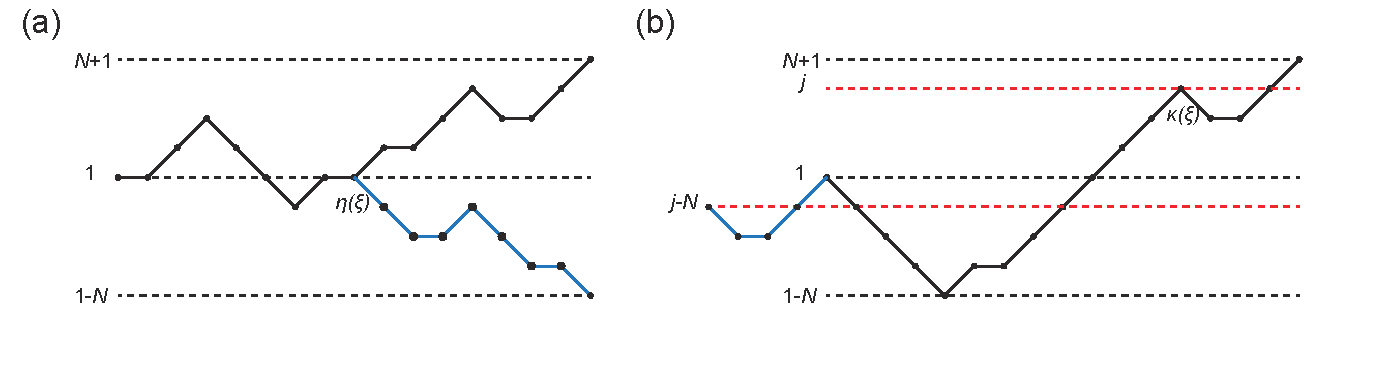
\includegraphics[scale=0.7]{chart/brokenlinegraph.pdf}
	\caption{$\xi$ 的轨迹对应的折线图。(a)第一种类型的轨迹映射(b)第二种类型的轨迹映射}
	\label{fig:linechart}
\end{figure}
\begin{lemma}\label{lemma:BiBjCiCj}
	对任意 $i,j\in S$,有
	\begin{equation*}
		B^i\left(\tilde{k}\right)=B^j\left(\tilde{k}\right)=C^i\left(\tilde{k}\right)=C^j\left(\tilde{k}\right).
	\end{equation*}
	成立。
\end{lemma}

\begin{proof}
    下面证明中令 $i=1$,这并不影响命题的适用性。我们只需证 $B^1(\tilde{k})=C^1(\tilde{k})=B^j(\tilde{k})$。首先证明 $B^1(\tilde{k})=C^1(\tilde{k})$。该系统是单环马氏链,$\xi$ 的每条轨迹可以被看作是一个折线图(见图 \ref{fig:linechart}(a))。在$m$时刻,折线在状态 $i$ 处的水平移动表示环 $(i)$ 形成。折线从状态$i+1$ ($-j$) 到状态 $i$ ($1-j$) 的每次上升(下降)对应于环$(i, i+1)$的形成。(其中的加减运算的结果都会经过模 $N$ 运算后的结果)。
    对任意轨迹 $\xi=(\xi_m)_{0\le m\le n}\in G^{1,+}(1,0,\tilde{k})$,令 $\eta(\xi)=\max\{m: 0\le m\le n-1,\xi_m=1\}$。由定义 $G^{1,+}(1,0,\tilde{k})$,轨迹 $(\xi_m)_{0\le m\le n}$ 在时间 $n$ 和状态 $N+1$ 到达集合 $\{N+1,1-N\}$。那么构造 $\xi$ 对应的轨迹 $\tilde{\xi}$(见图 \ref{fig:linechart} (a))
	\begin{equation*}
		\tilde{\xi}_m
		:=\left\{\begin{aligned}
			&\xi_m,    && \text{if } 0\le m\le \eta(\xi),\\
			&\xi_{n+\eta(\xi)-m},    && \text{if }\eta(\xi)<m\le n.\\
		\end{aligned}\right.
	\end{equation*}
    所有 $(\xi_m)_{0\le m\le \eta(\xi)}$ 中形成的环,在$(\tilde{\xi}_m)_{0\le m\le \eta(\xi)}$中也有形成。折线轨迹 $(\xi_m)_{\eta(\xi)\le m\le n}$ 在状态 $i$ 时刻 $m$ 的水平移动对应于 $(\tilde{\xi}_m)_{\eta(\xi)\le m\le n}$ 在状态 $i-N$ 时刻 $n+\eta(\xi)-m$ 的水平移动。
    类似的,折线轨迹 $(\xi_m)_{\eta(\xi)\le m\le n}$ 在时间 $m$ 从状态$i+1$ 到状态 $i$ 的下落对应于 $(\tilde{\xi}_m)_{\eta(\xi)\le m\le n}$ 在时间 $n+\eta(\xi)-m$ 从状态 $i-N$ 到状态 $i+1-N$ 的下落。那么所有 $(\xi_m)_{0\le m\le \eta(\xi)}$中形成的单状态和两状态环在 $(\tilde{\xi}_m)_{0\le m\le \eta(\xi)}$ 中也有形成。
    而且,轨迹 $(\tilde{\xi}_m)_{0\le m\le n}$ 在时刻 $n$ 和状态 $1-N$第一次到达集合 $\{N+1,1-N\}$,这说明轨迹 $(\tilde{\xi}_m)_{0\le m\le n}$ 最后形成的环是 $(1,N,\cdots,2)$,使得 $\tilde{\xi}\in G^{1,-}(0,1,\tilde{k})$。那么 $\xi\to \tilde{\xi}$ 是从 $G^{1,+}(1,0,\tilde{k})$ 到 $G^{1,-}(0,1,\tilde{k})$ 的一一映射,这说明 $B^1(\tilde{k})=C^1(\tilde{k})$。

    现在已经证明 $B^1(\tilde{k})=B^j(\tilde{k})$。对任意 $\tilde{k}$,令 $\tilde{G}^i(\tilde{k})$ 为满足下列所有条件轨道的集合,1)从状态$i$出发的$n$步轨道($n=N+\sum_{i \in S}(k^i+2k^{i,i+1})$)是。2)经过边 $\langle i,i\rangle$ $k^i$ 次。3)经过边 $\langle i,i+1\rangle$ $k^{i,i+1}$ 次。4)在时刻 $n$ 第一次到达状态 $N+i$。

    我们已经阐明对任意 $j\in S$,$|\tilde{G}^1(\tilde{k})|=|\tilde{G}^j(\tilde{k})|$ 成立。对任意轨迹 $\xi=(\xi_m)_{0\le m\le n}\in \tilde{G}^{1}(\tilde{k})$,令 $\kappa^j(\xi)=\min\{m: 0\le m\le n,\xi_k=j\}$,$\xi$也可以被视为折线图(见图 \ref{fig:linechart} (b))。我们构造 $\xi$ 对应的轨迹 $\tilde{\xi}$ 为:
    \begin{equation*}
		\tilde{\xi}_k
		:=\left\{\begin{aligned}
			&\xi_{\kappa(\xi)+k},    && \text{if } 0\le k\le n-\kappa(\xi),\\
			&\xi_{k+\kappa(\xi)-n},    && \text{if }n-\kappa(\xi)<k\le n.\\
		\end{aligned}\right.
	\end{equation*}
    因此 $(\tilde{\xi}_m)_{0\le m\le n} \in \tilde{G}^i(\tilde{k})$。既然 $\kappa(\xi)$ 是 $\xi$ 第一次到达状态 $j$,这说明 $n$ 也是 $\tilde{\xi}$ 第一次到达状态 $j+N$,那么$\tilde{\xi}\in \tilde{G}^j(\tilde{k})$。显然,$\xi\to\tilde{\xi}$ 是从 $\tilde{G}^1(\tilde{k})$ 到 $\tilde{G}^j(\tilde{k})$的一一映射,这说明 $|\tilde{G}^1(\tilde{k})|=|\tilde{G}^j(\tilde{k})|$。
    对轨迹 $\xi\in\tilde{G}^j(\tilde{k})$,环 $(i)$,$(i,i+1)$,$(1,\cdots,N)$,$(1,N,\cdots,2)$ 分别形成 $k^i$,$k^{i,i+1}-l$,$l+1$,$l$ 次,其中 $l\le \min_{i\in S}k^{i,i+1}$ 依赖于 $\xi$。既然 $\xi$ 在 $n$ 时到达状态 $N+j$ ,那么 $\xi$ 形成的最后一个环是 $(1,\cdots,N)$,因此
	\begin{equation*}
		\tilde{G}^j\left(\tilde{k}\right)=\bigsqcup_{l=0}^{\min_{i\in S}k^{i,i+1}}G^{j,+}\left(l+1,l,k^1,\cdots,k^N,k^{12}-l,\cdots,k^{N1}-l\right),
	\end{equation*}
	\begin{equation}\label{equality for AjBj}
		\left|\tilde{G}^j\left(\tilde{k}\right)\right|=\sum_{l=1}^{\min_{i\in S}k^{i,i+1}}\left|G^{j,+}\left(l+1,l,k^1,\cdots,k^N,k^{12}-l,\cdots,k^{N1}-l\right)\right|+B^j\left(\tilde{k}\right).
	\end{equation}
	下面用归纳法证明 $B^1(\tilde{k})=B^j(\tilde{k})$。当 $\min_{i\in S}k^{i,i+1}=0$, 通过方程 \eqref{equality for AjBj},可以得到 
    \begin{equation*}
		B^1(\tilde{k})=|\tilde{G}^1(\tilde{k})|=|\tilde{G}^j(\tilde{k})|=B^j(\tilde{k}).
	\end{equation*} 
	假设等式对 $\min_{i\in S}k^{i,i+1}\le m$ 成立。当 $\min_{i\in S}k^{i,i+1}=m+1$ 时,固定 $1\le l\le \min_{i\in S}k^{i,i+1}$,并且令 $\xi\in G^{j,+}_n(l+1,l,k^1,\cdots,k^N,k^{12}-l,\cdots,k^{N1}-l)$。那么轨迹 $\xi$ 可以被分为 $2l+1$ 个子轨迹, 每一个子轨迹最后形成的环是 $(1,\cdots,N)$ 或 $(1,N,\cdots,2)$。注意到最后一个环 $(1,\cdots,N)$ is $\binom{2l}{l}$ 形成前,在状态 1 处插入 $l$ 环 $(1,\cdots,N)$ 和 $l$ 个环 $(1,N,\cdots,2)$ 的排列数是 $\binom{2l}{l}$。固定剩余的环的分区(即 $\sum_{s=1}^{2l+1}\tilde{k}_s=(k^1,\cdots,k^N,k^{12}-l,\cdots,k^{N1}-l)$),因为对任意 $i$ 和 $\tilde{k}$,插入方式的排列数为 $\prod_{s=1}^{2l+1}B^j(\tilde{k}_s)$,那么:
	\begin{align*}
		&\;\left|G^{j,+}\left(l+1,l,k^1,\cdots,k^N,k^{12}-l,\cdots,k^{N1}-l\right)\right|\\
		=&\;\binom{2l}{l}\sum_{\sum_{s=1}^{2l+1}\tilde{k}_s=(k^1,\cdots,k^N,k^{12}-l,\cdots,k^{N1}-l)}\prod_{s=1}^{2l+1}B^j\left(\tilde{k}_s\right).
	\end{align*}
	
	因为 $l\ge 1$,,所以有 $B^1(\tilde{k}_s)=B^j(\tilde{k}_s)$,那么:
	\begin{align*}
		&\left|G^{1,+}\left(l+1,l,k^1,\cdots,k^N,k^{12}-l,\cdots,k^{N1}-l\right)\right|\\
		=&\left|G^{j,+}\left(l+1,l,k^1,\cdots,k^N,k^{12}-l,\cdots,k^{N1}-l\right)\right|.
	\end{align*}
	依据式 \eqref{equality for AjBj},可知$B^1(\tilde{k})=B^j(\tilde{k})$。最后通过归纳法,完成证明。
\end{proof}
\begin{proposition}\label{proposition:E Gin}
	考虑任意 $1\le i,j\le N$, $k\in\mathbb{N}^{2N+2}$ 和导出链 $\eta$,可得下面三条结论:
	\begin{itemize}
		\item[(i)] 
		\begin{equation}\label{EGin}
			\left|G^i\left(k^+,k^-,\tilde{k}\right)\right|=\left|G^i\left(k^-,k^+,\tilde{k}\right)\right|.
		\end{equation}
		\item[(ii)] 
		\begin{equation}\label{E Gi1cdotsNn}
			\left|G^{i,+}(k)\right|=\left|G^{j,+}(k)\right|,\qquad\left|G^{i,-}(k)\right|=\left|G^{j,-}(k)\right|.
		\end{equation}
		\item[(iii)]  
		\begin{equation}\label{EGetan}
			\left|G^{\eta}\left(k^+,k^-,\tilde{k}\right)\right|=\left|G^{\eta}\left(k^-,k^+,\tilde{k}\right)\right|.
		\end{equation}
	\end{itemize}
\end{proposition}
\begin{proof}
	(1) 首先考虑在状态 $i$ 插入环 $k^+$ 个环 $(1,\cdots,N)$ 和 $k^-$ 个环  $(1,N,\cdots,2)$,那么相应的排列数为 $\binom{k^++k^-}{k^+}$。接下来把剩余的环 (i.e. $k^i$ 个环 $(i)$ 和 $k^{i,i+1}$ 个环 $(i,i+1)$)分为 $k^++k^-+1$ 个部分。将剩余环的分区固定为 $\sum_{s=1}^{k^++k^-+1}\tilde{k}_s=\tilde{k}$。通过引理 \ref{lemma:BiBjCiCj},插入的数量为:
	\begin{equation*}
		\left[\prod_{s=1}^{k^++k^-}B^i(\tilde{k}_s)\right]\left|G^i(0,0,\tilde{k}_{k^++k^-+1})\right|,
	\end{equation*}
	其中 $B^i(\tilde{k}_s)$ 是在第 $(s-1)$ 个和 第 $s-$ 个 $N$ 状态环之间插入 $\tilde{k}_s$ 个环的排列数,且 $|G^i(0,0,\tilde{k}_{k^++k^-+1})|$ 是在第 $(k^++k^-)$ 个 $N$ 状态环之后插入 $\tilde{k}_{k^++k^-+1}$ 个环的排列数。由 $\sum_{s=1}^{k^++k^-+1}\tilde{k}_s=\tilde{k}$,可以得到:
	\begin{align}\label{E Gin}
		\left|G^i\left(k^+,k^-,\tilde{k}\right)\right|=\binom{k^++k^-}{k^+}\sum_{\sum_{s=1}^{k^++k^-+1}\tilde{k}_s=\tilde{k}}\left[\prod_{s=1}^{k^++k^-}B^i\left(\tilde{k}_s\right)\right]\left|G^i\left(0,0,\tilde{k}_{k^++k^-+1}\right)\right|.
	\end{align}
	注意到 \eqref{E Gin} 是关于 $k^+$ 和 $k^-$ 对称的,故(1)证毕。
	
	(ii) 上面证明了 \eqref{E Gi1cdotsNn} 中的第一个等式,第二个等式的证明与其相似。但是这里考虑的是轨迹 $\xi\in G^{i,+}_n(k)$,最后的环是 $(1,\cdots,N)$,只需在状态 $i$ 处插入 $k^+-1$ 个环 $(1,\cdots,N)$ 和 $k^-$ 个环 $(1,N,\cdots,2)$,可以得到:
	\begin{align*}
		&\left|G^{i,+}\left(k\right)\right|=\binom{k^++k^--1}{k^+-1}\sum_{\sum_{s=1}^{k^++k^-}\tilde{k}_s=\tilde{k}}\prod_{s=1}^{k^++k^-}B^i\left(\tilde{k}_s\right)\\
		&\qquad\qquad=\binom{k^++k^--1}{k^+-1}\sum_{\sum_{s=1}^{k^++k^-}\tilde{k}_s=\tilde{k}}\prod_{s=1}^{k^++k^-}B^j\left(\tilde{k}_s\right)=\left|G^{j,+}\left(k\right)\right|,
	\end{align*}
	其中第二步出自引理 ~\ref{lemma:BiBjCiCj}。

	(iii) 记 $\eta=[i_0,i_1,\cdots,i_t]$,首先把所有的环分为 $t+1$ 个部分,固定一部分为 $\sum_{s=0}^t k_s=k$,那么 $k^c_s$ 个环 $c$ ($\forall c\in\mathcal{C}$) 将被插入在 $\eta$ 的状态 $i_s$ ($0\le s\le t$)。那么可插入方式的数量为 $\prod_{s=0}^t |G^{i_s}(k_s)|$。由 $\sum_{s=0}^t k_s=k$,可以得到
	\begin{equation*}
		\left|G^{\eta}(k)\right|=\sum_{\sum_{s=0}^t k_s=k}\prod_{s=0}^t \left|G^{i_s}(k_s)\right|.
	\end{equation*}
	注意到对任意分区 $\sum_{s=0}^t k_s=k$,可知 $\sum_{s=0}^t (k_s^-,k_s^+,\tilde{k}_s)=(k^-,k^+,\tilde{k})$ 是 $(k^-,k^+,\tilde{k})$ 的一个分区。那么由方程 \eqref{EGin},可得:
	\begin{align*}
		\left|G^{\eta}(k^-,k^+,\tilde{k})\right|=&\sum_{\sum_{s=0}^t (k_s^-,k_s^+,\tilde{k}_s)=(k^-,k^+,\tilde{k})}\prod_{s=0}^t \left|G^{i_s}(k_s^-,k_s^+,\tilde{k}_s)\right|\\
		=&\sum_{\sum_{s=0}^t k_s=k}\prod_{s=0}^t \left|G^{i_s}(k_s)\right|=\left|G^{\eta}(k)\right|.
	\end{align*}
\end{proof}
下面将陈述 $| (G^i(k)|$ 和 $|G^{i,c}(k)|$ 的相关性。
\\
\begin{lemma}\label{lemma:E G1cnk}
	对任意 $k\in \mathbb{N}^{2N+2}$ 和 $i\in S$,令 $c\in \mathcal{C}$ 包含状态 $i$ 的环,那么:
	\begin{align*}
		\left|G^{i,c}(k)\right| = \frac{k^c}{k_i}\left|G^i(k)\right|.
	\end{align*}
\end{lemma}
\begin{proof}
	下面只证明 $i=1$ 时的情况,并不降低一般性。 回顾计算 $|G^1(k)|$ 的三个步骤。
	在第一个步骤中固定最后一个环 $c$,并且把排列数转换为
	\begin{equation*}
		\frac{k^c}{k^{1}+k^{12}+k^{1N}+k^{+}+k^{-}}A_1.
	\end{equation*}
	第二,三个步骤不变。在这种情况下,轨迹形成的最后一个环是 $c$,这意味着:
	\begin{align*}
		\left|G^{1,c}(k)\right| = \frac{k^c}{k_1}\left|G^1(k)\right|.
	\end{align*}
\end{proof}
\begin{proposition}\label{corollary:rate function is unrelated to the starting state}
	$I_J$ 不依赖于初始分布的选择 $\xi$.
\end{proposition}
\begin{proof}
	记 $c=(1,\cdots,N)$ 或 $(1,N,\cdots,2)$,通过命题 ~\ref{proposition:E Gin} 和引理 ~\ref{lemma:E G1cnk},易知 $\log|G^1(k)|=\log|G^i(k)|+O(\log n)$,那么由式 \eqref{ratefunction},命题得证。
\end{proof}

%%%%%%%%%%%%%%%%%%%%%%%%%%%%%%%%%%%%%%%%%%%%%%%%%%%%%%%%%%%%%%%%%%%%%%%%%%%%%
\BiSubsection{大偏差原理的严格证明和速率函数的性质}{}

我们建立了经验LE环流大偏差原理,还要严格证明速率函数的水平集是紧的,也就是验证条件 \eqref{def1} 和 \eqref{def2}。下面给出经验LE环流大偏差原理的严格阐述:
\begin{theorem}\label{thm:LDP}
    单环马氏链的经验环流$(J^c_n)_{c\in\mathcal{C}}$满足大偏差原理,并且相应的速率函数$I_J:\mathcal{V}\to [0,\infty]$满足上式 \eqref{ratefunction}. 速率函数$I_J$满足有界性,连续性和凸性。并且,速率函数$I_J$并不依赖初始分布的选择。
\end{theorem}

这里把大偏差原理的证明 ~\ref{thm:LDP} 分为两部分。首先研究经验环流的速率函数的性质。回顾速率函数 $I_J:\mathcal{V}\to[0,\infty]$ 的形式为:
\begin{equation*}\label{ratefunction1}
	\begin{split}
		I_J(\nu) =&\; \left[h\left(\nu^{12}\right)+h\left(\nu^{1N}\right)
		+h\left(\nu^+\right)+h\left(\nu^-\right)-h\left(\nu^{12}+\nu^{1N}+\nu^++\nu^-\right)\right] \\
		&\;+\inf_{X\in V(\nu)}F_{\nu}(X)+\sum_{i\in S}\left[ h\left(\nu_i-\nu^i\right)+h\left(\nu^i\right)
		-h\left(\nu_i\right)\right]-\sum_{c\in\mathcal{C}}\nu^c\log\gamma^c\\
		:=&\;I_1(\nu)+I_2(\nu)+I_3(\nu)+I_4(\nu).
	\end{split}
\end{equation*}
\begin{proposition}\label{proposition:I}
	速率函数 $I_J$ 是有界,连续的凸函数。
\end{proposition}
\begin{proof}
	易知 $I_j$ 有界。首先证明 $I_J$ 连续。易知 $h$ 是定义在 $[0,\infty)$ 的连续函数。那么 $I_1$ 和 $I_3$ 是连续的。注意到  $I_4$ 是关于 $\nu$ 的连续函数,因此还需证明 $I_2$ 是连续函数。令 $Y(\nu)\in V(\nu)$ 是方程 \eqref{equations} 的解,由于 \eqref{equations} 是一个多项式方程组,因此易知 $Y(\nu)$ 是关于变量 $\nu$ 的连续函数。由于 $h$ 是连续的,根据 \eqref{formula:F},可得$\inf_{X\in V(\nu)}F_{\nu}(X)=F_{\nu}(Y(\nu))$ 是关于 $\nu$ 的连续函数。
	
	然后证明 $I_J$ 是凸函数。 回顾 log-sum 不等式,对任意 $a_{1},a_{2},b_{1},b_{2}\ge 0$,有:
	\begin{equation}\label{log sum inequality}
		(a_1+a_2)\log \frac{a_1+a_2}{b_1+b_2}\le a_{1}\log \frac{a_{1}}{b_{1}}+a_{2}\log \frac{a_{2}}{b_{2}} ,
	\end{equation}
	注意到
	\begin{equation}\label{I_1}
		I_1(\nu) = \nu^{12}\log\left(\frac{\nu^{12}}{\hat{\nu}}\right)+\nu^{1N}\log\left(\frac{\nu^{1N}}{\hat{\nu}}\right)+\nu^{+}\log\left(\frac{\nu^{+}}{\hat{\nu}}\right)+\nu^{-}\log\left(\frac{\nu^{-}}{\hat{\nu}}\right),
	\end{equation}
	其中 $\hat{\nu}=\nu^{12}+\nu^{1N}+\nu^++\nu^-$。对任意满足 $\alpha+\beta=1$ 的 $\alpha,\beta\ge 0$ 和 $\nu,\mu\in \mathcal{V}$,通过log-sum 不等式 \eqref{log sum inequality},可以得到:
	\begin{equation*}
		(\alpha \nu^{12}+\beta \mu^{12})\log\left(\frac{\alpha \nu^{12}+\beta \mu^{12}}{\alpha \hat{\nu}+\beta \hat{\mu}}\right)\le \alpha\nu^{12}\log\left(\frac{\nu^{12}}{\hat{\nu}}\right)+\beta\mu^{12}\log\left(\frac{\mu^{12}}{\hat{\mu}}\right),
	\end{equation*}
	其中 $\hat{\mu}=\mu^{12}+\mu^{1N}+\mu^++\mu^-$。这说明 \eqref{I_1} 式的第一项的右边是关于 $\nu$ 的连续函数,同理,其他三项项的右边也是关于 $\nu$ 的连续函数。因此 $I_1(\nu)$ 是凸函数。同理,可以通过log-sum 不等式得到 $I_3(\nu)$也是凸函数。由于 $I_4(\nu)$ 是线性函数,那么也是凸函数,最后只需证明 $\inf_{X\in V(\nu)}F_{\nu}(X)$ 是凸函数。 把\eqref{formula:F} 重写为:
	\begin{align*}
		F_{\nu}(X)=&\;\sum_{i=2}^{N-1}\left[(x^{i-1}+\nu^+)\log\left(\frac{x^{i-1}+\nu^+}{x^{i-1}+x^i+\nu^+}\right)+x^i\log\left(\frac{x^{i}}{x^{i-1}+x^i+\nu^+}\right)\right]\\
		&\;+\sum_{i=2}^{N-1}\left[y^i\log\left(\frac{y^{i}}{y^{i}+y^{i+1}+\nu^-}\right)+(y^{i+1}+\nu^-)\log\left(\frac{y^{i+1}+\nu^-}{y^{i}+y^{i+1}+\nu^-}\right)\right]\\
		:=&\;\sum_{i=2}^{N-1}[A_1^i(\nu,X)+A_2^i(\nu,X)+A_3^i(\nu,X)+A_4^i(\nu,X)].
	\end{align*}
	既然对任意 $X=(x^i,y^i)\in V(\nu)$ 和 $Z=(z^i,w^i)\in V(\mu)$,有 $\alpha X+\beta Z\in V(\alpha\nu+\beta\mu)$。那么通过 log-sum 不等式,可得:
	\begin{align*}
		&\;A_1^i(\alpha\nu+\beta \mu,\alpha X+\beta Y)\\
		=&\;(\alpha x^{i-1}+\beta z^{i-1}+\alpha\nu^++\beta \mu^+ )\log\left(\frac{\alpha x^{i-1}+\beta z^{i-1}+\alpha\nu^++\beta \mu^+}{\alpha x^{i-1}+\alpha x^i+\beta z^{i-1}+\beta z^i+\alpha\nu^++\beta \mu^+}\right)\\
		=&\;(\alpha (x^{i-1}+\nu^+)+\beta (z^{i-1}+ \mu^+) )\log\left(\frac{\alpha (x^{i-1}+\nu^+)+\beta (z^{i-1}+ \mu^+)}{\alpha (x^{i-1}+ x^i+\nu^+)+\beta (z^{i-1}+ z^i+ \mu^+)}\right)\\
		\le &\; \alpha (x^{i-1}+\nu^+)\log\left(\frac{x^{i-1}+\nu^+}{x^{i-1}+ x^i+\nu^+}\right)+\beta (z^{i-1}+ \mu^+)\log\left(\frac{z^{i-1}+ \mu^+}{z^{i-1}+ z^i+ \mu^+}\right)\\
		=&\;\alpha A^i_1(\nu,X)+\beta A^i_1(\mu,Y).
	\end{align*}
	同理, 对任意 $j=2,3,4$ 有 $A^i_j(\alpha \nu+\beta \mu,\alpha X+\beta Y)\le \alpha A^i_j(\nu,X)+\beta A^i_j (\mu,Y)$。这说明
	\begin{equation*}
		F_{\alpha \nu+\beta \mu}(\alpha X+\beta Y)\le \alpha F_{\nu}(X)+\beta F_{\mu}(Y).
	\end{equation*}
	最后,对 $F_{\nu}$ 和 $F_{\mu}$ 取极小,可以得到:
	\begin{align*}
		\inf_{Z\in V(\alpha\nu+\beta\mu)}F_{\alpha\nu+\beta\mu}( Z)\le\alpha \inf_{X\in V(\nu)} F_{\nu}(X)+\beta \inf_{Y\in V(\mu)} F_{\mu}(Y).
	\end{align*}
	证毕。
\end{proof}
下面给出 LDP 原理的严格证明。
\\
\begin{proposition}\label{theorem:LDP}
	经验环流 $(J^c_n)_{c\in\mathcal{C}}$ 满足速率为 $n$ 的大偏差原理,并且相应的速率函数为 $I_J:\mathcal{V}\to [0,\infty]$。此外,它的上界可以为:对任意集合 $\Gamma \subset \mathcal{V}$,有:
	\begin{align}\label{upper bound}
		\varlimsup_{n\to+\infty}\;
		\frac 1n \log \mathbb  P \left( (J^c_n)_{c\in \mathcal{C}} \in \Gamma \right)
		\le -\inf_{\nu\in \Gamma} I_J(\nu).
	\end{align}
\end{proposition}
\begin{proof}
记
\begin{align}\label{set:K_n}
K_n := \left\{(k^c)_{c\in \mathcal{C}}\in \mathbb{N}^{2N+2}: \sum_{c \in \mathcal{C}} k^{c} |c| =n \right\}.
\end{align}
接下来的证明还会假设马氏链从状态 1 出发。那么,对任意 $k=(k^c)_{c\in\mathcal{C}}\in K_n$,由 \eqref{joint} 式,可得:
\begin{align}\label{Jnxi}
\mathbb{P}_1\left(J^c_{n}= \frac{k^c}{n},\ \forall c\in \mathcal{C}\right)
= |G_n(k)| \prod_{c\in\mathcal{C}}\left(\gamma^c\right)^{k^c},
\end{align}
记 $\mu_n(k) = k/n\in\mathcal{V}$。对任意 $\Gamma\subset \mathcal{V}$,令
\begin{align*}
Q_n(\Gamma) = \max_{k\in K_n: \mu_n(k) \in \Gamma}
\mathbb{P}_1\left(J^c_{n} = \frac{k^c}{n},\ \forall c\in\mathcal{C}\right).
\end{align*}
显然有:
\begin{align}\label{Qn gamma}
	Q_n(\Gamma)
	\le \mathbb{P}_1\left(J_{n} \in \Gamma\right)
	\le |K_n| Q_n(\Gamma).
\end{align}
易知 $|K_n| \le (2N+2)(n+1)^{2N+3}$,那么由公式 \eqref{Jnxi},\eqref{Qn gamma},\eqref{log A1},\eqref{log A3},和\eqref{log A2},可得:
\begin{equation}\label{1 n log P}
	\begin{split}
	\frac{1}{n}\log\mathbb{P}_1\left(J_{n} \in \Gamma\right)=&O\left(\frac{\log n}{n}\right)+\frac{1}{n}\log Q_n(\Gamma)\\
	=&O\left(\frac{\log n}{n}\right)+\max_{k\in K_n: \mu_n(k) \in \Gamma}\left[\frac{1}{n}\log |G_{n}(k)|+\sum_{c \in \mathcal{C}}\frac{k_c}{n}\log \gamma^c\right]\\
	=&O\left(\frac{\log n}{n}\right)-\min_{k\in K_n: \mu_n(k) \in \Gamma}I_J\left(\mu_{n}(k)\right).
	\end{split}
\end{equation}
由于 $\cup_{n\in\mathbb{N}} \{\mu_{n}(k):k\in K_n\}$ 在 $\mathcal{V}$ 中稠密,且 $\nu\to I_J(\nu)$ 在 $\mathcal{V}$ 中连续(见命题 \ref{proposition:I}),这保证了对每个 $\nu\in \mathcal{V}$,存在序列 $(k_n)_{n\in \mathbb{N}}$,使得:
\begin{equation*}
\lim_{n\to\infty} \|\mu_{n}(k_n)-\nu\| = 0, \qquad \lim_{n\to\infty} I_J\left(\mu_{n}(k_n)\right) = I_J(\nu).
\end{equation*}
那么对任意开集 $U\subset \mathcal{V}$
\begin{equation*}
\varlimsup_{n\to\infty}\min_{k\in K_n: \mu_n(k) \in U}I_J\left(\mu_{n}(k)\right)\le I_J(\nu),\quad\forall\nu\in U.
\end{equation*}
对 $\nu\in U$ 取极小,可得:
\begin{equation}\label{varlimsup}
\varlimsup_{n\to\infty}\min_{k\in K_n: \mu_n(k) \in U}I_J\left(\mu_{n}(k)\right)\le \inf_{\nu\in U}I_J(\nu).
\end{equation}
结合 \eqref{1 n log P} 和 \eqref{varlimsup},可得大偏差原理的下界 \eqref{def1}。此外,对任意$\Gamma \subset \mathcal{V}$,同理可得反向的不等式,即
\begin{equation}\label{varliminf}
\varliminf_{n\to\infty}\min_{k\in K_n: \mu_n(k) \in \Gamma}I_J\left(\mu_{n}(k)\right)\ge \inf_{\nu\in \Gamma}I_J(\nu).
\end{equation}
结合 \eqref{1 n log P} 和 \eqref{varliminf},可得大偏差原理的上界 \eqref{def2}。
\end{proof}
%%%%%%%%%%%%%%%%%%%%%%%%%%%%%%%%%%%%%%%%%%%%%%%%%%%%%%%%%%%%%%%%%%%%%%%%%%%%%%%%%%%%

%%%%%%%%%%%%%%%%%%%%%%%%%%%%%%%%%%%%%%%%%%%%%%%%%%%%%%%%%%%%%%%%%%%%%%
\BiSubsection{大偏差速率函数的简化形式}{}
一般单环马氏链的速率函数表达式 \eqref{ratefunction} 十分复杂。不过,针对下面两种特殊情况,速率函数 $I_J$ 形式将会被简化,1)三状态马氏链。2)状态 1 到状态 N 的转移概率为 0 的单环马氏系统。

回顾速率函数 $I_J:\mathcal{V}\to[0,\infty]$ 的公式为:
\begin{equation*}\label{ratefunction1}
	\begin{split}
		I_J(\nu) =&\; \left[h\left(\nu^{12}\right)+h\left(\nu^{1N}\right)
		+h\left(\nu^+\right)+h\left(\nu^-\right)-h\left(\nu^{12}+\nu^{1N}+\nu^++\nu^-\right)\right] \\
		&\;+\inf_{X\in V(\nu)}F_{\nu}(X)+\sum_{i\in S}\left[ h\left(\nu_i-\nu^i\right)+h\left(\nu^i\right)
		-h\left(\nu_i\right)\right]-\sum_{c\in\mathcal{C}}\nu^c\log\gamma^c\\
		:=&\;I_1(\nu)+I_2(\nu)+I_3(\nu)+I_4(\nu).
	\end{split}
\end{equation*}
\begin{proposition}
三状态马氏链的速率函数为
\begin{align*}
I_J(\nu) =
\sum_{i\in S} \left[\nu^{i}\log \left(\frac{\nu^{i}/\nu_i}{J^i/J_i}\right) + (\nu_i - \nu^i)\log \left(\frac{(\nu_i - \nu^i)/\nu_i}{(J_i - J^i)/J_i} \right)
\right]
+ \sum_{c \in \mathcal{C}, |c|\neq 1} \nu^{c} \log \left(\frac{\nu^{c}/\tilde{\nu}}{J^c/\tilde{J}}\right).
\end{align*}
\end{proposition}
\begin{proof}
	易知 $X=(x^2,y^2)$ 为方程 \eqref{equations} 的解,其中
\begin{equation*}
	x^{2}=\frac{\nu^{23}\left(\nu^{12}+\nu^+\right)}{\nu^{12}+\nu^{13}+\nu^++\nu^-},\quad y^{2}=\frac{\nu^{23}\left(\nu^{13}+\nu^-\right)}{\nu^{12}+\nu^{13}+\nu^++\nu^-}.
\end{equation*}
根据引理 ~\ref{lemma:mininum}
\begin{equation*}\label{Fnu2}
I_2(\nu)=F_{\nu}(X)=\nu^{23}\log\frac{\nu^{23}}{\tilde{\nu}}+\left(\nu^{12}+\nu^{13}+\nu^++\nu^-\right)\log\frac{\tilde{\nu}-\nu^{23}}{\tilde{\nu}}.
\end{equation*}
那么通过计算,我们可以得到:
\begin{equation}\label{I1I2I3}
	I_1(\nu)+I_2(\nu)+I_3(\nu) = \sum_{i\in S} \left[\nu^{i}\log \frac{\nu^{i}}{\nu_i} + (\nu_i - \nu^i)\log \frac{\nu_i - \nu^i}{\nu_i} 
	\right]
	+ \sum_{c \in \mathcal{C}, |c|\neq 1} \nu^{c} \log \frac{\nu^{c}}{\tilde{\nu}}.
\end{equation}
回顾环流的表达 \cite[Theorem.1.3.3]{jiang2004mathematical},有
\begin{equation}\label{J+J-Jii+1}
J^+=\gamma^+\frac{1}{C},\quad J^-=\gamma^-\frac{1}{C},\quad J^{i,i+1}=\gamma^{i,i+1}\frac{1-p_{i-1,i-1}}{C}, \quad 1\le i\le 3,
\end{equation}
其中 $C=3+\sum_{i\in S}[p_{ii}p_{i+1,i+1}-p_{i,i+1}p_{i+1,i}-2(p_{ii}+p_{i+1,i+1})]$. 根据 \eqref{decomposition},
\begin{equation}\label{pij}
	p_{ij}=\frac{\sum_{c \ni \langle i,j\rangle}J^c}{\sum_{c\ni i}J^c}.
\end{equation}
结合 \eqref{J+J-Jii+1} 和 \eqref{pij},有:
\begin{equation}\label{nucgamma2}
	\begin{split}
		&\;\sum_{i \in S}\left[\nu^i\log\frac{J^i}{J_i}+\left(\nu_i-\nu^i\right)\log\frac{J_i-J^i}{J_i}\right]+ \sum_{c \in \mathcal{C}, |c|\neq 1} \nu^{c} \log \left(\frac{J^c}{\tilde{J}}\right)\\
		=&\;\sum_{i \in S}\left[\nu^i\log\frac{J^i}{J_i}+\nu^{i,i+1}\log\left(\left(1-\frac{J^i}{J_i}\right)\left(1-\frac{J^{i+1}}{J_{i+1}}\right)\frac{J^{i,i+1}}{\tilde{J}}\right)\right]\\
		&\;+\nu^+\log\left(\frac{J^+}{\tilde{J}}\prod_{i\in\mathcal{C}}\left(1-\frac{J^i}{J_i}\right)\right)+\nu^-\log\left(\frac{J^-}{\tilde{J}}\prod_{i\in\mathcal{C}}\left(1-\frac{J^i}{J_i}\right)\right)\\
		=&\;\sum_{c \in \mathcal{C}}\nu^c \log\gamma^c=-I_4(\nu).
	\end{split}
\end{equation}
结合 \eqref{I1I2I3} 和 \eqref{nucgamma2},得证。
\end{proof}
\begin{proposition}
	状态 1 到状态 N 的转移概率为 0 的单环马氏链的速率函数为:
	\begin{equation*}
		\begin{split}
			I_J(\nu) = \sum_{i\in S}\left[\nu^i\log\left(\frac{\nu^i/\nu_i}{J^i/J_i}\right)
			+\nu^{i,i+1}\log\left(\frac{\nu^{i,i+1}/\nu_i}{J^{i,i+1}/J_i}\right)+\left(\nu^{i-1,i}+\nu^+\right)\log\left(\frac{\left(\nu^{i-1,i}+\nu^+\right)/\nu_i}
			{\left(J^{i-1,i}+J^+\right)/J_i}\right)\right].
		\end{split}
	\end{equation*}
\end{proposition}
\begin{proof}
	在 $p_{1N}=0$ 的条件下,环 $(1,N)$ 和环 $(1,N,\cdots,2)$ 不会被形成。因此,可以得到\eqref{equation} 中的 $\nu^{1N}=\nu^{-}=0$ ,并且 $x^{i}=\nu^{i,i+1}$, $y^{i}=0$ 是方程 \eqref{equation}的解,那么
	\begin{equation*}
		I_2(\nu)=F_{\nu}(x^i,y^i)=\sum_{i=2}^{N-1}\left[-\lambda_{i}\nu^{i,i+1}+\nu^+\log\frac{\nu^{i-1,i}+\nu^+}{\nu^{i-1,i}+\nu^{i,i+1}+\nu^+}\right]+\nu^{12}\log\frac{\nu^{12}+\nu^+}{\nu^{12}+\nu^{23}+\nu^+},
	\end{equation*}
	其中 
	\begin{equation*}
		\lambda_i=-\log\left(\frac{\nu^{i,i+1}}{\nu^{i-1,i}+\nu^{i,i+1}+\nu^+}\,\frac{\nu^{i,i+1}+\nu^+}{\nu^{i,i+1}+\nu^{i+1,i+2}+\nu^+}\right).
	\end{equation*}
	通过 $\nu_i$ 的定义,有
	\begin{equation*}
		\nu_1=\nu^{1}+\nu^{12}+\nu^+,\quad \nu_i=\nu^i+\nu^{i-1,i}+\nu^{i,i+1}+\nu^+,\ 2\le i\le N-1,\quad \nu_N=\nu^N+\nu^{N-1,N}+\nu^+.
	\end{equation*} 
然后通过计算,可以得到:	
\begin{equation}\label{I1lack}
	I_1(\nu)=\nu^{12}\log\frac{\nu^{12}}{\nu_1-\nu^{12}}+\nu^+\log\frac{\nu^+}{\nu_1-\nu^1},
\end{equation}
	\begin{align}\label{I2lack}
	I_2(\nu)
	=\sum_{i=2}^{N}\left[\nu^{i,i+1}\log\frac{\nu^{i,i+1}}{\nu_i-\nu^i}+\nu^+\log\frac{\nu^{i-1,i}+\nu^+}{\nu_i-\nu^i}\right]+\sum_{i=1}^{N}\nu^{i,i+1}\log\frac{\nu^{i,i+1}+\nu^+}{\nu_{i+1}-\nu^{i+1}},
   \end{align}
和
	\begin{equation}\label{I3lack}
		\begin{split}
			I_3(\nu)=\sum_{i\in S}\left[\nu^i\log\frac{\nu^i}{\nu_i}+\nu^+\log\frac{\nu_i-\nu^i}{\nu_i}\right]+\sum_{i\in S}\nu^{i,i+1}\left(\log\frac{\nu_i-\nu^i}{\nu_i}
			+\log\frac{\nu_{i+1}-\nu^{i+1}}{\nu_{i+1}}\right).
		\end{split}
	\end{equation}
    根据 \eqref{pij},可得
	\begin{equation}\label{nucgammac}
		\begin{split}
			&\;\sum_{i \in S}\left[\nu^i\log\frac{J^i}{J_i}+\nu^{i,i+1}\log\frac{J^{i,i+1}}{J_i}+(\nu^{i-1,i}+\nu^+)\log\frac{J^{i-1,i}+J^+}{J_i}\right]\\
			=&\;\sum_{i \in S}\left[\nu^i\log\frac{J^i}{J_i}+\nu^{i,i+1}\log\frac{J^{i,i+1}(J^{i,i+1}+J^+)}{J_{i+1}J_i}\right]+\nu^+\log\frac{\prod_{i=1}^N\left(J^{i,i+1}+J^+\right)}{\prod_{i=1}^N J_i}\\
			=&\;\sum_{c \in \mathcal{C}}\nu^c \log\gamma^c=-I_4(\nu).
		\end{split}
	\end{equation}
	结合 \eqref{I1lack},\eqref{I2lack},\eqref{I3lack},和 \eqref{nucgammac},证毕。
\end{proof}
%%%%%%%%%%%%%%%%%%%%%%%%%%%%%%%%%%%%%%%%%%%%%%%%%%%%%%%%%%%%%%%%%%%%%%%%%

% 对于三状态马氏链,则速率函数可以化简为:(证明细节见 \ref{appendix:threestate})
% \begin{align*}
%     I_J(\nu) =
%     \sum_{i\in S} \left[\nu^{i}\log \left(\frac{\nu^{i}/\nu_i}{J^i/J_i}\right) + (\nu_i - \nu^i)\log \left(\frac{(\nu_i - \nu^i)/\nu_i}{(J_i - J^i)/J_i} \right)
%     \right]
%     + \sum_{c\in\mathcal{C},|c|\neq 1} \nu^{c} \log \left(\frac{\nu^{c}/\tilde{\nu}}{J^c/\tilde{J}}\right) ,
% \end{align*}
% 其中
% \begin{align*}
%     \tilde{\nu} &=\sum_{c\in\mathcal{C},|c|\neq 1}\nu^{c}
%     = \nu^{12}+\nu^{13}+\nu^{23}+\nu^++\nu^-,\\
%     \tilde{J} &=\sum_{c\in\mathcal{C},|c|\neq 1}J^{c}
%     = J^{12}+J^{13}+J^{23}+J^++J^-.
% \end{align*}
% 对于N状态单环马氏链,且$p_{1N}=0$,速率函数可以化简为(证明细节见 \ref{appendix:threestate}):
% \begin{equation}\label{lack}
%     \begin{split}
%         I_J(\nu) = \sum_{i\in S}\Bigg[&\;\nu^i\log\left(\frac{\nu^i/\nu_i}{J^i/J_i}\right)
%         +\nu^{i,i+1}\log\left(\frac{\nu^{i,i+1}/\nu_i}{J^{i,i+1}/J_i}\right)\\
%         &\;+\left(\nu^{i-1,i}+\nu^+\right)\log\left(\frac{\left(\nu^{i-1,i}+\nu^+\right)/\nu_i}
%         {\left(J^{i-1,i}+J^+\right)/J_i}\right)\Bigg].
%     \end{split}
% \end{equation}

注意到上述两种情况下的速率函数表达式更简单,形式更对称 \eqref{ratefunction},并且与初始状态的选择无关。这也进一步验证了定理\ref{thm:LDP}的相关结论。

LE经验环流$(J^{c}_n)_{c\in\mathcal{C}}$的大偏差原理结果可以直接应用到经验LE净环流$(\tilde{J}^{c}_n)_{c\in\mathcal{C}}$。对一状态和两状态马氏链$\tilde{J}^c_n = 0$且$\tilde{J}^+_n = -\ {J}^-_n$,只需要考虑环$(1, 2, \cdots ,N)$的经验净环流$\tilde{J}^+_n$。那么由收缩原理可以得到:
\begin{equation}\label{tilde I J}
	\begin{split}
		\mathbb{P}\left(\tilde{J}^{+}_n = x\right)
		&=\;\mathbb{P}\left(J^{+}_n-J^{-}_n = x\right)\\
		&=\;\sum_{\nu^{+}-\nu^{-}=x}\mathbb{P}\left(J^{c}_n=\nu^{c},\forall c\in\mathcal{C}\right)\\
		&\propto\sum_{\nu^{+}-\nu^{-}=x} e^{-nI_J(\nu)}.
	\end{split}
\end{equation}
由此说明$\tilde{J}^+_n$满足大偏差原理, 相应的速率函数$I_{\tilde{J}}$为:
\begin{equation*}
	I_{\tilde{J}}(x)=\inf_{\{\nu\in\mathcal{V}:\nu^{+}-\nu^{-}= x\}}I_J(\nu).
\end{equation*} 

\BiSection{一般马氏链的ST环流的大偏差}{}

文献 \cite{bertini2015flows} 中,已经有经验ST净环流的大偏差,和速率函数的对称性的相关介绍。接下来我们将着重研究经验ST环流的大偏差原理,涉及对经验测度内容可参考 \cite{den2000large}。

$n$时刻的对经验测度$R_n:E\rightarrow[0,1]$,可以定义为
\begin{equation*}
R_n(i,j) = \frac{1}{n}\sum_{m=1}^n1_{\{\xi_{m-1}=i,\xi_m=j\}},
\end{equation*}
显然$R_n(i,j)$表示边$\langle i,j\rangle$形成的速度。由于周期边界条件,对经验测度$R_n$处于空间
\begin{equation*}
\mathcal{M} = \left\{R:E\rightarrow[0,1]:\;\sum_{i,j\in S}R(i,j) = 1,\;
\sum_{j\in S}R(i,j)=\sum_{j\in S}R(j,i)\right\}.
\end{equation*}
众所周知,对经验测度满足下面的大偏差原理:
\begin{equation*}
\mathbb{P}(R_n(i,j)=R(i,j),\;\forall\langle i,j\rangle\in E)\propto e^{-nI_{\mathrm{pair}}(R)},\;\;\;n\to\infty,
\end{equation*}
上式中的速率函数$I_{\mathrm{pair}}:\mathcal{M}\rightarrow[0,\infty]$的表达式为
\begin{equation*}
I_{\mathrm{pair}}(R) = \sum_{\langle i,j\rangle\in E}R(i,j)\log\frac{R(i,j)}{R(i)p_{ij}}
\end{equation*}
其中$R(i)=\sum_{j\in S}R(i,j)$,可以看到,对经验测度的速率函数具有相对熵形式。给定生成树$T$,定义在空间$E$上的函数$H^{c_l}$为:
\begin{equation*}\label{cycle function2}
H^{c_l}(i,j)
    =\left\{\begin{aligned}
    1, &   && \text{if } \langle i,j\rangle \in c_l \text{ and }\langle i,j\rangle \in T, \text{ or } \langle i,j\rangle=l,\\
    -1,&   && \text{if } \langle i,j\rangle\notin c_l,\langle j,i\rangle \in c_l,\text{ and }\langle i,j\rangle \in T,\\
    0, &   && \text{otherwise}.\\
    \end{aligned}\right.
\end{equation*}
对经验测度可以被分解为下面ST环流的加权和:
\begin{equation*}
R_n(i,j) = \sum_{c_l\in\mathcal{L}}H^{c_l}(i,j)Q^{c_l}_n,
\end{equation*}
且由文献 \cite{kalpazidou2007cycle}可知,该分解是唯一的。也就是说,如果$R_n =\sum_{c_l \in \mathcal{L}\nu^{c_l}H^{c_l}}$,那么对任意$c_l \in \mathcal{L}$会有$\nu^{c_l}=Q_n^{c_l}$。由上述表达式的唯一性,可得:
\begin{equation*}
    \mathbb{P}(Q_n^{c_l}=\mu^{c_l},\;\forall c_l\in\mathcal{L})
    =\mathbb{P}\left(R_n(i,j)=\sum_{c_l\in\mathcal{L}}\mu^{c_l}H^{c_l}(i,j),\;\forall\langle i,j\rangle\in E\right)
    \propto e^{-n I_{\mathrm{pair}}\left(\sum_{c_l\in\mathcal{L}}\mu^{c_l}H^{c_l}\right)}.
\end{equation*}
这表明ST经验环流$(Q_n^{c_l})_{c_l\in\mathcal{L}}$满足大偏差原理,相应的速率函数$I_Q:\mathcal{M}\rightarrow[0,\infty]$为:
\begin{equation}\label{formula:I_Q}
I_Q(\mu)=I_{\mathrm{pair}}\left(\sum_{c_l\in\mathcal{L}}\mu^{c_l}H^{c_l}\right).
\end{equation}

目前,已经得到了单环马氏链经验环流的速率函数,和一般马氏链的经验ST环流的速率函数。我们将阐述两种速率函数的关系。前面也说过 ST 环流可以通过 LE 表示为$Q_n^{c_l} = \sum_{c\in\mathcal{C}}J^c_n1_{\{l\in c\}}$。从收缩原理中,可以得到:
\begin{align*}
	\mathbb{P}\left(Q_n^{c_l}=\mu^{c_l},\;\forall l\in\mathcal{L}\right)
	&= \mathbb{P}\left(\sum_{c\in\mathcal{C}}J^c_n1_{\{l\in c\}}=\mu^{c_l},\;\forall l\in\mathcal{L}\right)\\
	&= \sum_{\{\nu\in\mathcal{V}:\;\sum_c\nu^c1_{\{l\in c\}}=\mu^{c_l}\}}
	\mathbb{P}\left(J^c_n=\nu^c,\;\forall c\in\mathcal{C}\right)\\
	&\propto \sum_{\{\nu\in\mathcal{V}:\;\sum_c\nu^c1_{\{l\in c\}}=\mu^{c_l}\}}e^{-nI_J(\nu)}.
\end{align*}
这表明 LE 和 ST 经验环流的内在关系为:
\begin{equation*}
	I_Q(\mu) = \inf_{\{\nu\in\mathcal{V}:\;\sum_c\nu^c1_{\{l\in c\}}=\mu^{c_l}\}}I_J(\nu).
\end{equation*}
易知上式中的$I_Q$和式 \eqref{formula:I_Q} 中的一致,故该式的证明在此省略。

利用收缩原理也可以建立ST经验净环流$(\tilde{Q}^{c_l}_n)_{c_l\in\mathcal{L}}$的大偏差原理。对于一元环和二元环,ST经验净环流为0,因此只需考虑三元环或者多元环。令$\{c_{l_1}, c_{l_2}, \cdots, c_{l_s}\} \subset \mathcal{L}$ 表示基本集中所有三元环或者多元环,那么环$c$及相应的反环$c^-$只出现一次。再令$l_1$,$l_1-$,$l_2$,$l_2-$,$\cdots$,$l_s$,$l_s-$为基本集中环对应的弦。那么ST经验净环流$(\tilde{Q}^{c_{l_i}})_{1\le i\le s}$满足大偏差原理,且相应的速率函数$I_{\tilde{Q}}$为:
\begin{equation}\label{I_Q2}
	I_{\tilde{Q}}(x)=\inf_{\{\mu\in\mathcal{M}:\mu^{c_{l_{i}}}-\mu^{c_{l_{i}}-}= x_i,\forall 1\le i\le s\}}I_Q(\mu).
\end{equation}